\documentclass[aspectratio=169]{beamer}
\usetheme{Madrid}
\usecolortheme{beaver}
\usepackage[utf8]{inputenc}
\usepackage[T1]{fontenc}
\usepackage{tikz}
\usepackage{amssymb}
\usepackage{graphicx}
\setbeamertemplate{navigation symbols}{}
\setbeamercolor{title}{fg=white,bg=cyan!60!black}
\setbeamercolor{frametitle}{fg=white,bg=cyan!50!black}
\setbeamercolor{block title}{bg=cyan!15,fg=black}
\setbeamercolor{block body}{bg=cyan!5,fg=black}

\title{Block Arcade 2 — Motion \& Repeat}
\subtitle{"Repeat" blocks — do something several times without copy-pasting}
\author{ByteForge --- Grade 7 --- Game Maker --- Week Overview}
\date{}

\begin{document}

\begin{frame}
    \titlepage
\end{frame}

\begin{frame}{This Week's Plan}
    \begin{itemize}
        \item Lesson 1: Repeat 3 Times
        \item Lesson 2: Marching Line
        \item[$\bigstar$] BOSS --- Bouncing Sprite (\texttt{lessonBoss.tex})
    \end{itemize}
\end{frame}

\begin{frame}{Real-World Example}
    \Large
    A marching band or a row of parked cars, evenly spaced — the spacing pattern (each one a fixed distance from the last) is the exact "loop + changing variable" idea. Minecraft building a straight fence or a row of torches is the same repeat pattern, just done by hand instead of by a loop.
\end{frame}


\begin{frame}{Image}
    \begin{center}
    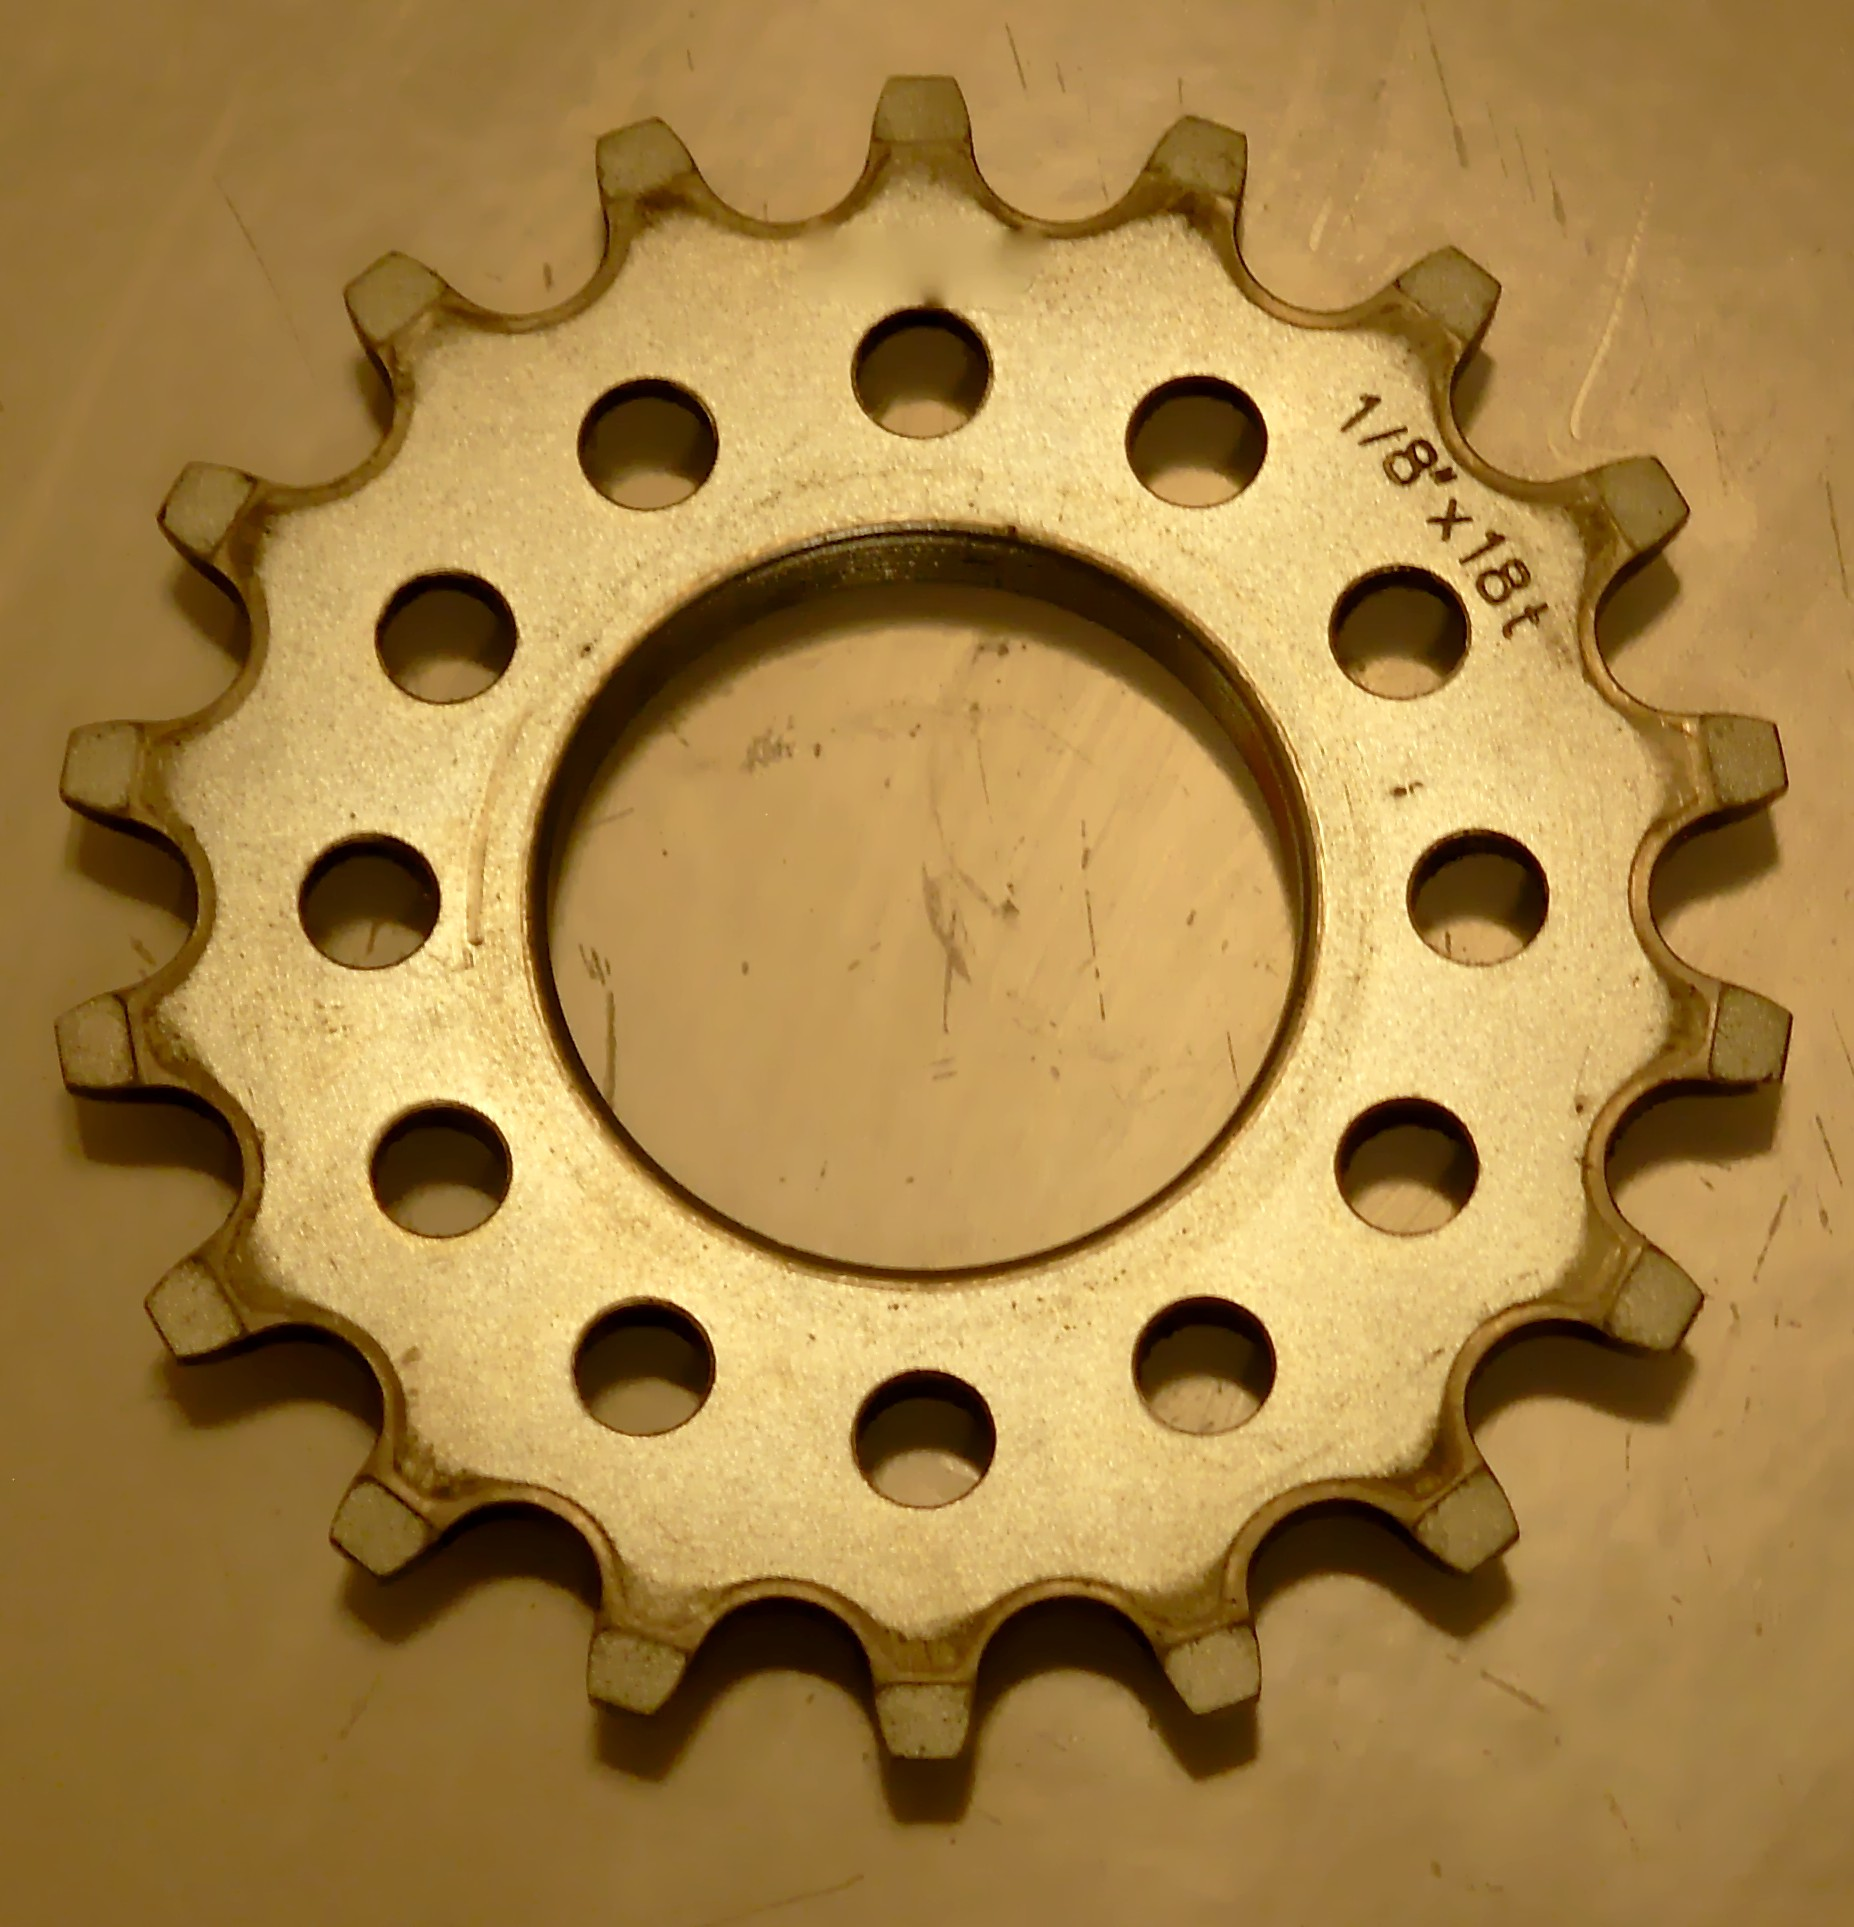
\includegraphics[width=0.55\textwidth]{../images/gear.jpg}

    \small Fixed gear cog — John Reaves, public domain, via Wikimedia Commons
    \end{center}
\end{frame}

\begin{frame}{Let Them Discover}
    \Large
    Watch any 2D platformer character walk for 10 seconds. Roughly how many times does it "step" a tiny bit? Movement that looks smooth is secretly hundreds of small repeats — try to spot the individual frames.
\end{frame}

\begin{frame}{Files in This Folder}
    \small
    \begin{itemize}
        \item \texttt{lesson1.tex} --- Repeat 3 Times
        \item \texttt{lesson2.tex} --- Marching Line
        \item \texttt{lessonBoss.tex} --- BOSS: Bouncing Sprite
    \end{itemize}
    \vspace{0.5em}
    \normalsize Each lesson file is its own short deck --- open the one for
    the specific day you're teaching, not this whole overview.
\end{frame}

\end{document}
